% Imporditud: tools/import_eksperimendid.py
% Allikas: Eesti füüsikaolümpiaadi eksperimendi ülesannete
%   kogu (Rael Kalda, 2023), ülesanne Ü173, lahendus L173.
\setAuthor{Jaan Kalda}
\setRound{piirkonnavoor}
\setYear{2017}
\setNumber{G E2}
\setDifficulty{5}
\setTopic{staatika}
\setVahendid{mõned spagetikõrred, kaks tikutoosi, kaks tuntud massiga joonlauda (m = . . . )}
\setPunktid{12}
\setAllikas{Eksperimendi kogu Ü173, lahendus lk 131}
\setLahendusseis{kasitsi}

\prob{Spagett}
Kui painutatud spagett jagada mõtteliselt kaheks osaks, siis need kaks osa mõjutavad üksteist jõumomendiga T , mis sõltub spageti kõverusraadiusest R mõtteliste osade eralduspunktis. Hooke'i seaduse analoogi saab kirja panna valemina

T = k/R,

kus k on võrdetegur, mis sõltub spageti materjalist ja jämedusest. Leidke võrdetegur k teile antud spageti jaoks.
\begin{center}
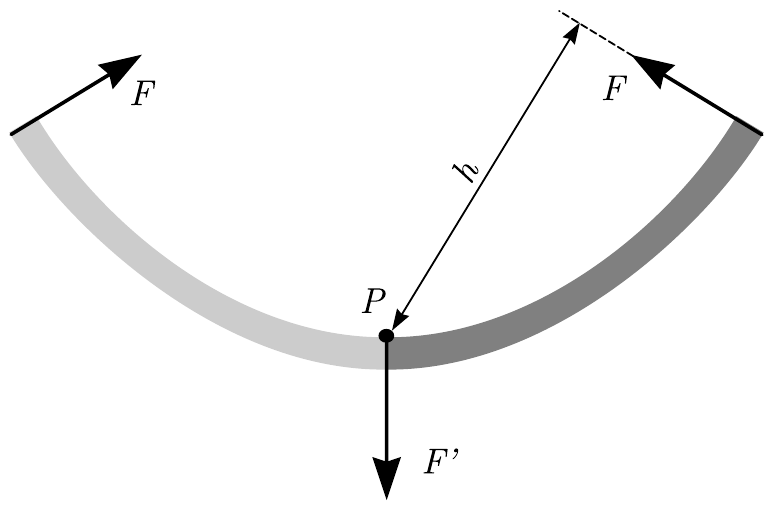
\includegraphics[width=0.55\linewidth]{2017-v2g-ge2-yl.png}
\end{center}
\textit{Vihje:} kui painutada spagetti kolme jõu abil nagu näidatud joonisel, siis parempoolne jõud F mõjutab paremat spagetipoolt punkti P suhtes jõumomendiga F h ning selle tasakaalustab vasaku spagetipoole poolt avaldatav jõumoment T = k/R, kus R on spageti kõverusraadius punktis P . Kõverusraadiuse leidmiseks punktis P eeldage lihtsustatult, et spagett on ringjoone kaar.

\hint

\solu
\textit{Lahendus on kogumikus lk 131. Siia ei ole seda veel ümber kirjutatud, sest originaalis on tabel või joonis, mis PDF-i tekstikihist loetavalt välja ei tule.}
\probend
